\documentclass[12pt,a4paper]{article}
\usepackage{amsmath,amscd,amsbsy,amssymb,latexsym,url,bm,amsthm}
\usepackage{epsfig,graphicx,subfigure}
\usepackage{enumitem,balance}
\usepackage{wrapfig}
\usepackage{mathrsfs,euscript}
\usepackage[usenames]{xcolor}
\usepackage{hyperref}
\usepackage[vlined,ruled,linesnumbered]{algorithm2e}
\usepackage{float}
\usepackage{multirow}
\usepackage{array}
\hypersetup{colorlinks=true,linkcolor=black}


\hypersetup{colorlinks=true,linkcolor=blue}

\newtheorem{theorem}{Theorem}
\newtheorem{lemma}[theorem]{Lemma}
\newtheorem{proposition}[theorem]{Proposition}
\newtheorem{corollary}[theorem]{Corollary}
\newtheorem{exercise}{Exercise}
\newtheorem*{solution}{Solution}
\newtheorem{definition}{Definition}
\theoremstyle{definition}



\renewcommand{\thefootnote}{\fnsymbol{footnote}}

\newcommand{\postscript}[2]
{\setlength{\epsfxsize}{#2\hsize}
	\centerline{\epsfbox{#1}}}

\renewcommand{\baselinestretch}{1.0}

\setlength{\oddsidemargin}{-0.365in}
\setlength{\evensidemargin}{-0.365in}
\setlength{\topmargin}{-0.3in}
\setlength{\headheight}{0in}
\setlength{\headsep}{0in}
\setlength{\textheight}{10.1in}
\setlength{\textwidth}{7in}
\makeatletter \renewenvironment{proof}[1][Proof] {\par\pushQED{\qed}\normalfont\topsep6\p@\@plus6\p@\relax\trivlist\item[\hskip\labelsep\bfseries#1\@addpunct{.}]\ignorespaces}{\popQED\endtrivlist\@endpefalse} \makeatother
\makeatletter
\renewenvironment{solution}[1][Solution] {\par\pushQED{\qed}\normalfont\topsep6\p@\@plus6\p@\relax\trivlist\item[\hskip\labelsep\bfseries#1\@addpunct{.}]\ignorespaces}{\popQED\endtrivlist\@endpefalse} \makeatother

\begin{document}
	\noindent
	
	%========================================================================
	\noindent\framebox[\linewidth]{\shortstack[c]{
			\Large{\textbf{Lab10-Turing Machine}}\vspace{1mm}\\
			Algorithm and Complexity (CS214), Xiaofeng Gao, Spring 2020.}}
	\begin{center}
		\footnotesize{\color{red}$*$ If there is any problem, please contact TA Yiming Liu. }
		
		\footnotesize{\color{blue}$*$ Name: Yulong Hui  \quad Student ID: 518030910059 \quad Email: qinchuanhuiyulong@sjtu.edu.cn}
	\end{center}
	
	\begin{enumerate}
		
		\item
		Design a one-tape TM $M$ that computes the function $f(x, y) = x \mod y$, where $x$ and $y$ are positive integers ($x > y$). The alphabet is $\{1, 0, \Box, \triangleright, \triangleleft\}$, and the inputs are $x$ 1's, $\Box$ and $y$ 1's. Below is the initial configuration for input $x=7$ and $y=3$. The result $z=f(x, y)$ should also be represented in the form of $z$ 1's on the tape with the pattern of $\triangleright 111 \cdots 111 \triangleleft$.
		\begin{center}
			\begin{tabular}{ll|c|c|c|c|c|c|c|c|c|c|c|c|c|c}
				& \multicolumn{14}{c}{Initial Configuration} \\ [5pt]
				\cline{2-16}
				& & $\triangleright$ &  1  & 1 & 1 & 1 & 1 & 1 & 1 & $\Box$ & 1 & 1 & 1 & $ \triangleleft$ & \\
				\cline{2-16}
				%				\multicolumn{2}{c}{} & \multicolumn{1}{c}{$\uparrow$} & \multicolumn{11}{c}{} \\ [-4px]
				\multicolumn{2}{c}{} & \multicolumn{1}{c}{$q_S$} & \multicolumn{11}{c}{}	
			\end{tabular}
		\end{center}
		
		\begin{enumerate}
			\item
			Please describe your design and then write the specifications of $M$ in the form like $\langle q_S, \triangleright \rangle \rightarrow \langle q_1, \triangleright,  R\rangle$. Explain the transition functions in detail.
			
			\item
			Please draw the state transition diagram.
			
			\item
			Show briefly and clearly the whole process from initial to final configurations for input $x = 7$ and $y = 3$. You may start like this:
			$$(q_s,\underline{\triangleright}  1  1  1  1  1  1  1  \Box 1  1  1   \triangleleft)
			\vdash (q_1,\triangleright  \underline{1}  1  1  1  1  1  1  \Box 1  1  1   \triangleleft)
			\vdash^* (q_1,\triangleright  1  1  1  1  1  1  1  \underline{\Box} 1  1  1   \triangleleft)
			\vdash (q_2,\triangleright  1  1  1  1  1  1  1  \Box \underline{1}  1  1   \triangleleft)$$
			
			\par{\color{blue}(Note that for simplicity, we write $(q_1,\triangleright  \underline{1}  1  1  1  1  1  1  \Box 1  1  1   \triangleleft)\vdash^* (q_1,\triangleright  1  1  1  1  1  1  1  \underline{\Box} 1  1  1   \triangleleft)$ if the corresponding transaction repeats on multiple inputs with the same state.)}
			
		\end{enumerate}
		
		~\\
		\textbf{Solution.}
		\begin{enumerate}
			\item In every loop, we minus both $x$ and $y$ by $1$. To implement it, we can replace $1$ in $x$-sequence with $\triangleright$, and replace $1$ in $y$-sequence with $0$. 
			
			When all cells of $y$ become $0$, we change it into the original value of $y$ which means fill the y-cells with 1. 
			
			Finally, $x$ will become $0$. Assuming $y$ becomes $y^\prime$ , then $x\mod y= z =y-y^\prime$, and $z$ is equal to the number of $0$.
			
			The transition funtions are as follows:
			
			\textbf{Start:}
			
			$\langle q_S,\triangleright\rangle\rightarrow\langle q_1,\triangleright,R\rangle$
			
			\textbf{Step 1: $x=x-1$}
			
			$\langle q_1,1\rangle\rightarrow\langle q_2,\triangleright,R\rangle$
			
			$\langle q_1,\Box\rangle\rightarrow\langle q_6,\triangleright,R\rangle$
			
			\textbf{Step 2:} Move from $x$  to $y$
			
			$\langle q_2,1\rangle\rightarrow\langle q_2,1,R\rangle$
			
			$\langle q_2,\Box\rangle\rightarrow\langle q_3,\Box,R\rangle$
			
			\textbf{Step 3: }$y=y-1$
			
			$\langle q_3,0\rangle\rightarrow\langle q_3,0,R\rangle$
			
			$\langle q_3,\triangleleft\rangle\rightarrow\langle q_4,\triangleleft,L\rangle$
			
			$\langle q_3,1\rangle\rightarrow\langle q_5,0,L\rangle$
			
			\textbf{Step 4:} If $y$ has become 0 before minus, fill the cells with 1. 
			
			$\langle q_4,0\rangle\rightarrow\langle q_4,1,L\rangle$
			
			$\langle q_4,\Box\rangle\rightarrow\langle q_3,\Box,R\rangle$
			
			\textbf{Step 5:} Move from $y$ to $x$
			
			$\langle q_5,0\rangle\rightarrow\langle q_5,0,L\rangle$
			
			$\langle q_5,\Box\rangle\rightarrow\langle q_5,\Box,L\rangle$
			
			$\langle q_5,1\rangle\rightarrow\langle q_5,1,L\rangle$
			
			$\langle q_5,\triangleright\rangle\rightarrow\langle q_1,\triangleright,R\rangle$
			
			\textbf{Step 6: }Get result
			
			$\langle q_6,0\rangle\rightarrow\langle q_6,1,R\rangle$
			
			$\langle q_6,1\rangle\rightarrow\langle q_t,\triangleleft,S\rangle$
			
			$q_t$: halt
			
			\quad\par
			Step-1  sets the first $1$ in $x$ to $\triangleright$ which means $x=x-1$. If the symbol at current location is $\Box$, then there is no '$1$' left, so we change the $\Box$ into $\triangleright$ and move right, and go to step 6 to get the result.
			
			Then we use Step 2 to move from $x$-sequence to $y$-sequence .
			
			In step 3, we minus $y$ by 1. We move right until meeting the first $1$ and then we change it to $0$. But if  $y$ equals to $0$ (we meet $\triangleleft$ before meeting  $1$), we jump to step $4$, and fill all the cells with $1$. Otherwise, we go to step 5.
			
			In step 5, we move from $y$-sequence to $x$-sequence.
			
			In step 6, we change all '$0$' into '$1$' in $y$-sequence,  Then change the first previous $1$ into $\triangleleft$ as an ending signal of the result.
			
			\item The state transition diagram is as follows:
			
			\begin{figure}[!htbp]
				\centering
				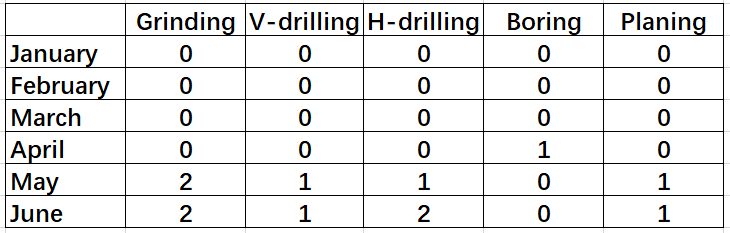
\includegraphics[scale= 0.8]{1.png}
				\caption{Transition Diagram.} \label{Fig-Conflict}
			\end{figure}
			
			\item The whole process is as follows:
			
			$$q_1,\underline{\triangleright} 1111111\Box111\triangleleft$$
			$$q_1,\triangleright\underline{1}111111\Box111\triangleleft$$
			$$q_2,\triangleright\triangleright\underline{1}11111\Box111\triangleleft$$
			$$q_2,\triangleright\triangleright111111\underline{\Box}111\triangleleft$$
			$$q_3,\triangleright\triangleright111111\Box\underline{1}11\triangleleft$$
			$$q_5\triangleright\triangleright111111\underline{\Box}011\triangleleft$$
			$$q_5\triangleright\triangleright11111\underline{1}\Box011\triangleleft$$
			$$q_5,\triangleright\triangleright\underline{1}11111\Box011\triangleleft$$
			$$q_5,\triangleright\underline{\triangleright}111111\Box011\triangleleft$$
			$$q_1,\triangleright\triangleright\underline{1}11111\Box011\triangleleft$$
			$$q_2\triangleright\triangleright\triangleright\underline{1}1111\Box011\triangleleft$$
			$$q_2,\triangleright\triangleright\triangleright11111\underline{\Box}011\triangleleft$$
			$$q_3,\triangleright\triangleright\triangleright11111\Box\underline{0}11\triangleleft$$
			$$q_3,\triangleright\triangleright\triangleright11111\Box0\underline{1}1\triangleleft$$
			$$q_5,\triangleright\triangleright\triangleright11111\Box\underline{0}01\triangleleft$$
			$$q_5,\triangleright\triangleright\triangleright11111\underline{\Box}001\triangleleft$$
			$$q_5,\triangleright\triangleright\triangleright1111\underline{1}\Box001\triangleleft$$
			$$q_5,\triangleright\triangleright\triangleright\underline{1}1111\Box001\triangleleft$$
			$$q_5,\triangleright\triangleright\underline{\triangleright}11111\Box001\triangleleft$$
			$$q_1,\triangleright\triangleright\triangleright\underline{1}1111\Box001\triangleleft$$
			$$q_2,\triangleright\triangleright\triangleright\triangleright\underline{1}111\Box001\triangleleft$$
			$$q_2,\triangleright\triangleright\triangleright\triangleright1111\underline{\Box}001\triangleleft$$
			$$q_3,\triangleright\triangleright\triangleright\triangleright1111\Box\underline{0}01\triangleleft$$
			$$q_3,\triangleright\triangleright\triangleright\triangleright1111\Box0\underline{0}1\triangleleft$$
			$$q_3,\triangleright\triangleright\triangleright\triangleright1111\Box00\underline{1}\triangleleft$$
			$$q_5,\triangleright\triangleright\triangleright\triangleright1111\Box0\underline{0}0\triangleleft$$
			$$q_5,\triangleright\triangleright\triangleright\triangleright1111\underline{\Box}000\triangleleft$$
			$$q_5,\triangleright\triangleright\triangleright\triangleright111\underline{1}\Box000\triangleleft$$
			$$q_5,\triangleright\triangleright\triangleright\triangleright\underline{1}111\Box000\triangleleft$$
			$$q_5,\triangleright\triangleright\triangleright\underline{\triangleright}1111\Box000\triangleleft$$
			$$q_1,\triangleright\triangleright\triangleright\triangleright\underline{1}111\Box000\triangleleft$$
			$$q_2,\triangleright\triangleright\triangleright\triangleright\triangleright\underline{1}11\Box000\triangleleft$$
			$$q_2,\triangleright\triangleright\triangleright\triangleright\triangleright111\underline{\Box}000\triangleleft$$
			$$q_3,\triangleright\triangleright\triangleright\triangleright\triangleright111\Box\underline{0}00\triangleleft$$
			$$q_3,\triangleright\triangleright\triangleright\triangleright\triangleright111\Box000\underline{\triangleleft}$$
			$$q_4,\triangleright\triangleright\triangleright\triangleright\triangleright111\Box00\underline{0}\triangleleft$$
			$$q_4,\triangleright\triangleright\triangleright\triangleright\triangleright111\Box0\underline{0}1\triangleleft$$
			$$q_4,\triangleright\triangleright\triangleright\triangleright\triangleright111\underline{\Box}111\triangleleft$$
			$$q_3,\triangleright\triangleright\triangleright\triangleright\triangleright111\Box\underline{1}11\triangleleft$$
			$$q_5,\triangleright\triangleright\triangleright\triangleright\triangleright111\underline{\Box}011\triangleleft$$
			$$q_5,\triangleright\triangleright\triangleright\triangleright\triangleright11\underline{1}\Box011\triangleleft$$
			$$q_5,\triangleright\triangleright\triangleright\triangleright\underline{\triangleright}111\Box011\triangleleft$$
			$$q_1,\triangleright\triangleright\triangleright\triangleright\triangleright\underline{1}11\Box011\triangleleft$$
			$$q_2,\triangleright\triangleright\triangleright\triangleright\triangleright\triangleright\underline{1}1\Box011\triangleleft$$
			$$q_2,\triangleright\triangleright\triangleright\triangleright\triangleright\triangleright11\underline{\Box}011\triangleleft$$
			$$q_3,\triangleright\triangleright\triangleright\triangleright\triangleright\triangleright11\Box\underline{0}11\triangleleft$$
			$$q_3,\triangleright\triangleright\triangleright\triangleright\triangleright\triangleright11\Box0\underline{1}1\triangleleft$$
			$$q_5,\triangleright\triangleright\triangleright\triangleright\triangleright\triangleright11\Box\underline{0}01\triangleleft$$
			$$q_5,\triangleright\triangleright\triangleright\triangleright\triangleright\triangleright11\underline{\Box}001\triangleleft$$
			$$q_5,\triangleright\triangleright\triangleright\triangleright\triangleright\triangleright1\underline{1}\Box001\triangleleft$$
			$$q_5,\triangleright\triangleright\triangleright\triangleright\triangleright\underline{\triangleright}11\Box001\triangleleft$$
			$$q_1,\triangleright\triangleright\triangleright\triangleright\triangleright\triangleright\underline{1}1\Box001\triangleleft$$
			$$q_2,\triangleright\triangleright\triangleright\triangleright\triangleright\triangleright\triangleright\underline{1}\Box001\triangleleft$$
			$$q_2,\triangleright\triangleright\triangleright\triangleright\triangleright\triangleright\triangleright1\underline{\Box}001\triangleleft$$
			$$q_3,\triangleright\triangleright\triangleright\triangleright\triangleright\triangleright\triangleright1\Box\underline{0}01\triangleleft$$
			$$q_3,\triangleright\triangleright\triangleright\triangleright\triangleright\triangleright\triangleright1\Box0\underline{0}1\triangleleft$$
			$$q_3,\triangleright\triangleright\triangleright\triangleright\triangleright\triangleright\triangleright1\Box00\underline{1}\triangleleft$$
			$$q_5,\triangleright\triangleright\triangleright\triangleright\triangleright\triangleright\triangleright1\Box0\underline{0}0\triangleleft$$
			$$q_5,\triangleright\triangleright\triangleright\triangleright\triangleright\triangleright\triangleright1\underline{\Box}000\triangleleft$$
			$$q_5,\triangleright\triangleright\triangleright\triangleright\triangleright\triangleright\triangleright\underline{1}\Box000\triangleleft$$
			$$q_5,\triangleright\triangleright\triangleright\triangleright\triangleright\triangleright\underline{\triangleright}1\Box000\triangleleft$$
			$$q_1\triangleright\triangleright\triangleright\triangleright\triangleright\triangleright\triangleright\underline{1}\Box000\triangleleft$$
			$$q_2,\triangleright\triangleright\triangleright\triangleright\triangleright\triangleright\triangleright\triangleright\underline{\Box}000\triangleleft$$
			$$q_3,\triangleright\triangleright\triangleright\triangleright\triangleright\triangleright\triangleright\triangleright\Box\underline{0}00\triangleleft$$
			$$q_3,\triangleright\triangleright\triangleright\triangleright\triangleright\triangleright\triangleright\triangleright\Box000\underline{\triangleleft}$$
			$$q_4,\triangleright\triangleright\triangleright\triangleright\triangleright\triangleright\triangleright\triangleright\Box00\underline{0}\triangleleft$$
			$$q_4,\triangleright\triangleright\triangleright\triangleright\triangleright\triangleright\triangleright\triangleright\Box0\underline{0}1\triangleleft$$
			$$q_4,\triangleright\triangleright\triangleright\triangleright\triangleright\triangleright\triangleright\triangleright\Box\underline{0}11\triangleleft$$
			$$q_4,\triangleright\triangleright\triangleright\triangleright\triangleright\triangleright\triangleright\triangleright\underline{\Box}111\triangleleft$$
			$$q_3,\triangleright\triangleright\triangleright\triangleright\triangleright\triangleright\triangleright\triangleright\Box\underline{1}11\triangleleft$$
			$$q_5,\triangleright\triangleright\triangleright\triangleright\triangleright\triangleright\triangleright\triangleright\underline{\Box}011\triangleleft$$
			$$q_5,\triangleright\triangleright\triangleright\triangleright\triangleright\triangleright\triangleright\underline{\triangleright}\Box011\triangleleft$$
			$$q_1,\triangleright\triangleright\triangleright\triangleright\triangleright\triangleright\triangleright\triangleright\underline{\Box}011\triangleleft$$
			$$q_6,\triangleright\triangleright\triangleright\triangleright\triangleright\triangleright\triangleright\triangleright\triangleright\underline{0}11\triangleleft$$
			$$q_6,\triangleright\triangleright\triangleright\triangleright\triangleright\triangleright\triangleright\triangleright\triangleright1\underline{1}1\triangleleft$$
			$$q_t,\triangleright\triangleright\triangleright\triangleright\triangleright\triangleright\triangleright\triangleright\triangleright1\underline{\triangleleft}1\triangleleft$$
			
			
		\end{enumerate}
		
		
		\item Assume there's a Turing Machine $M$ using alphabet $\Gamma :\{ \triangleright, \Box, a, b, \cdots, z\}$. We can simulate $M$ by a Turing Machine $\tilde{M}$ using alphabet $\tilde{\Gamma }:\{ \triangleright, \Box, 0, 1\}$. Please transform the instruction $\langle q, i \rangle \rightarrow \langle q',j, R\rangle$ in $M$ into its corresponding form in $\tilde{M}$.
		
		\begin{solution}
			In  $\tilde{M}$, we will use 5 symbols to represent a letter, like: $00001$ means $a$, and  $11010$ means $z$. Then, we will use 5 $\Box$ to represent one $\Box$, because $\Box$ may be rewritten by a letter and we should offer enough space. And, we can just use a $\triangleright$ as same as in Turing Machine $M$.
			
			We use $p$ to represent the stages of TM $\tilde{M}$, and, we can deal with three kinds of instruction separately.
			
			\textbf{First. }In $\langle q,i\rangle\rightarrow \langle q,j,R\rangle$, if $i$ is $\triangleright$ then $j$ should also be $\triangleright$, because $\triangleright$ always means the signal of beginning and it should not be changed.
			Then $\langle q,\triangleright\rangle \rightarrow \langle q',\triangleright,R\rangle $ can be transformed as $\langle p,\triangleright\rangle \rightarrow \langle p',\triangleright,R\rangle $
			
			\textbf{Second. }In  $\langle q,i\rangle\rightarrow \langle q,j,R\rangle$, if $i$ is $\Box$:
			
			Then, if $j$ is still $\Box$, then 
			$\langle q,\Box \rangle \rightarrow \langle q',\Box ,R\rangle $ can be transformed as:
			
			$\langle p,\Box \rangle \rightarrow \langle p_2,\Box,R \rangle $
			
			$\langle p_2,\Box \rangle \rightarrow \langle p_3,\Box,R \rangle $
			
			$\langle p_3,\Box \rangle \rightarrow \langle p_4,\Box,R \rangle $
			
			$\langle p_4,\Box \rangle \rightarrow \langle p_5,\Box,R \rangle $
			
			$\langle p_5,\Box \rangle \rightarrow \langle p',\Box,R \rangle $
			
			
			Else, j is a letter.We take $c$ as an example and other letters are similar to that. ($c$ can be transformed as $00011$) 
			
			Then, $\langle q_c,\Box \rangle \rightarrow \langle q',c ,R\rangle $ can be transformed as:
			
			$\langle p_c,\Box \rangle \rightarrow \langle p_{c2},0,R \rangle $
			
			$\langle p_{c2},\Box \rangle \rightarrow \langle p_{c3},0,R \rangle $
			
			$\langle p_{c3},\Box \rangle \rightarrow \langle p_{c4},0,R \rangle $
			
			$\langle p_{c4},\Box \rangle \rightarrow \langle p_{c5},1,R \rangle $
			
			$\langle p_{c5},\Box \rangle \rightarrow \langle p',1,R \rangle $
			
			\textbf{Third }In  $\langle q,i\rangle\rightarrow \langle q,j,R\rangle$, if $i$ is a letter, and we take $c$ as an example and other letters are similar to that. ($c$ can be transformed as $00011$)  :
			
			
			$\langle q,i \rangle \rightarrow \langle q',j ,R\rangle $ can be transformed:
			
			The following instructions are used to find out the corresponding letter.
			
			$\langle p,0 \rangle \rightarrow \langle p_0,0,R \rangle $
			
			$\langle p_0,0 \rangle \rightarrow \langle p_{00},0,R \rangle $
			
			$\langle p_{00},0 \rangle \rightarrow \langle p_{000},0,R \rangle $
			
			$\langle p_{000},1 \rangle \rightarrow \langle p_{0001},1,R \rangle $
			
			$\langle p_{0001},1 \rangle \rightarrow \langle p_{c},1,S \rangle $
			
			The following instructions are used to rewrite the symbol from $c$ to $j$.
			
			(a) If $j$ is $\Box$, then
			
			$\langle p_{c},1 \rangle \rightarrow \langle p_{c4},\Box,L \rangle $
			
			$\langle p_{c4},1 \rangle \rightarrow \langle p_{c3},\Box,L \rangle $
			
			$\langle p_{c3},0 \rangle \rightarrow \langle p_{c2},\Box,L \rangle $
			
			$\langle p_{c2},0 \rangle \rightarrow \langle p_{c1},\Box,L \rangle $
			
			$\langle p_{c1},\Box \rangle \rightarrow \langle p'_1,\Box,S \rangle $
			
			(b) If $j$ is letter '$d$' of $00010$, then
			
			$\langle p_{c},1 \rangle \rightarrow \langle p_{c4},0,L \rangle $
			
			$\langle p_{c4},1 \rangle \rightarrow \langle p_{c3},1,L \rangle $
			
			$\langle p_{c3},0 \rangle \rightarrow \langle p_{c2},0,L \rangle $
			
			$\langle p_{c2},0 \rangle \rightarrow \langle p_{c1},0,L \rangle $
			
			$\langle p_{c1},\Box \rangle \rightarrow \langle p'_1,0,S \rangle $
			
			Finally, the following instructions are used to relocate at the next letter ($X$ means any one of the symbols).
			
			$\langle p'_1, X \rangle \rightarrow \langle p'_2,X,R \rangle $
			
			$\langle p'_2,X \rangle \rightarrow \langle p'_3,X,R \rangle $
			
			$\langle p'_3,X \rangle \rightarrow \langle p'_4,X,R \rangle $
			
			$\langle p'_4,X \rangle \rightarrow \langle p'_5,X,R \rangle $
			
			$\langle p'_5,X \rangle \rightarrow \langle p',X,R \rangle $
			
			
		\end{solution}
		
		\item \textbf{Wireless Data Broadcast System.}
		In a Wireless Data Broadcast System (WDBS), data items are repeatedly broadcasted in cycle on different channels. Denote $D = \{d_1, d_2,\cdots, d_k\}$ as data items, each $d_i$ with length $l_i$ (as time units), and $\mathbf{C}=\{C_1, C_2, \cdots, C_n\}$ as broadcasting channels. Fig.~\ref{Fig-Broadcast} illustrates a WDBS with 25 data items and 4 channels. Once a channel finishes broadcasting current cycle, it will repeat these data again as a new cycle. E.g., a possible broadcasting sequence of $C_1$ could be \{$d_6$, $d_{12}$, $d_1$, $d_{18}$, $d_7$, $d_6$, $d_{12}$, $d_1$, $d_{18}$, $d_7$, $\cdots$\}
		
		\begin{figure}[h]
			\centering
			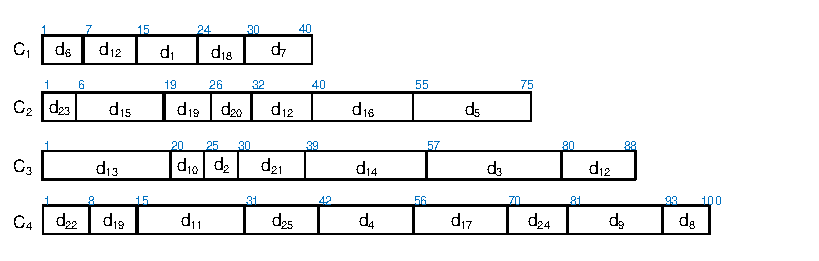
\includegraphics[scale=1]{Fig-Broadcast.pdf}
			\caption{An Example Scenario of Wireless Data Broadcast System.} \label{Fig-Broadcast}
		\end{figure}
		
		If a mobile client requires a subset of data items $D_q \subseteq D$ from this WDBS, he/she must access onto one channel, wait for the appearance of one required item, and switch to another channel if necessary. Each ``switch'' requires one time slot. For example, Lucien wants to download $\{d_1, d_3, d_5\}$, as shown in Fig.~\ref{Fig-Access}. He firstly accesses onto $C_1$ at time slot 1, then download $d_1$, $d_3$ respectively during time slots 2 to 5, and then switch to $C_3$ at time slot 6 (note that he cannot download $d_5$ from $C_2$ because of the switch constraint), and download $d_5$ during time slots 7 to 8. We define \emph{access latency} as the period when a client starts downloading, till the time he/she finishes. As a result, the overall access latency for Lucien is 7 in this example.
		
		\begin{figure}[!htbp]
			\centering
			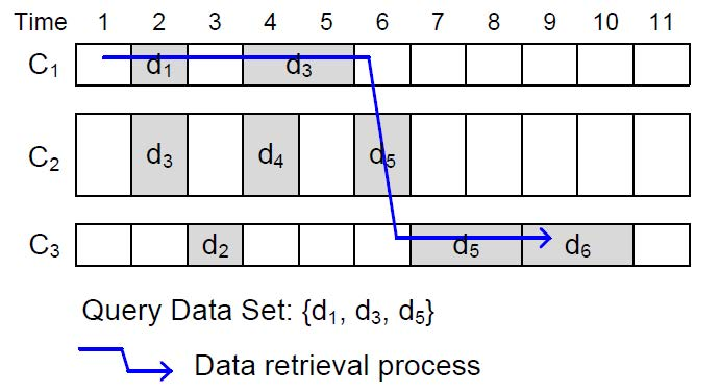
\includegraphics[scale= 0.5]{Fig-Access.pdf}
			\caption{An Example Scenario of Query of a Client.} \label{Fig-Access}
		\end{figure}
		
		Each operation (download/wait/switch) needs energy consumption. To conserve energy, a client hopes to use minimum amount of energy to download all required items in $D_q$, which means that he/she waits to minimize both access latency and switch numbers. Unfortunately, these two objectives conflict with each other naturally. Fig.~\ref{Fig-Conflict} exhibits such a scenario. To download $D_q=\{d_1, d_2, d_3, d_4\}$, if we start from $C_2$, in Option 1 we can switch to $C_1$ for $d_1$ immediately after downloading $d_3$, return back to $C_2$ for $d_4$, and to $C_1$ again for $d_2$. Such option costs 3 switches and 7 access latency. While in Option 2, we stay at $C_2$ lazily for $d_3$ and $d_4$, and then switch to $C_1$ for $d_2$ and $d_1$. Such option costs 1 switches and 12 access latency.
		
		
		\begin{figure}[!htbp]
			\centering
			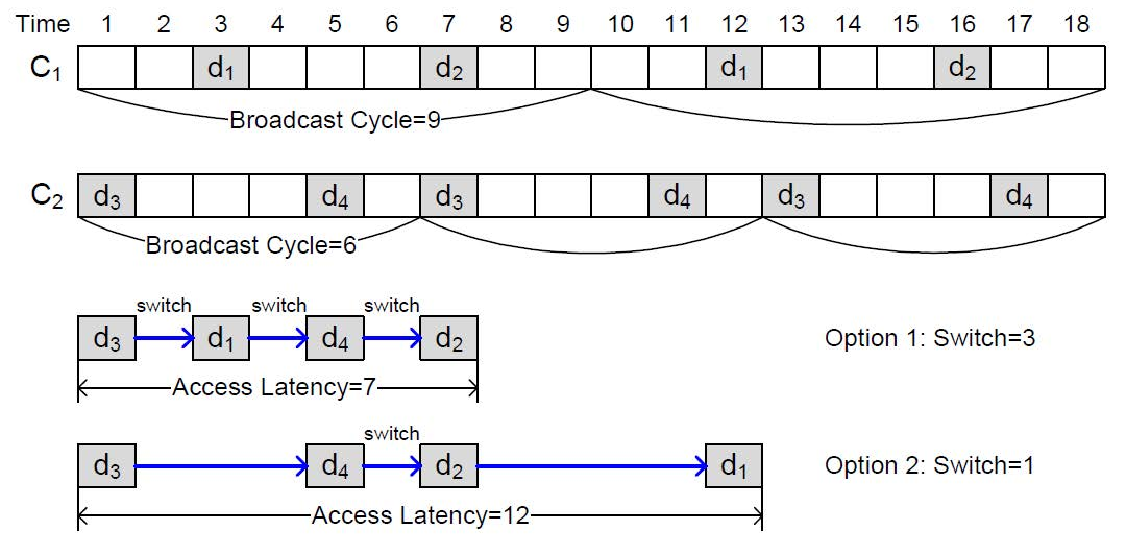
\includegraphics[scale= 0.5]{Fig-Conflict.pdf}
			\caption{Confliction between Access Latency and Switch Number.} \label{Fig-Conflict}
		\end{figure}
		
		Once we want to minimize two conflictive objectives simultaneously, we have three possible ways (similar as Segmented Least Squares told in Dynamic Programming Lecture). Now it is your turn to complete the formulation of this optimization, we name it as Minimum Constraint Data Retrieval Problem (MCDR), with the following sub-questions.
		\begin{enumerate}
			\item If we add an additional switch parameter $h$, please define the MCDR (Version 1) completely as a search problem.
			\item If we add an additional latency parameter $t$, please define the MCDR (Version 2) completely as a search problem.
			\item If we set dimensional parameters $\alpha$ to switch number, and $\beta$ to access latency, we can combine two objectives together linearly as a new concept ``cost''. Please define the Minimum Cost Data Retrieval Problem (MCDR, Version 3) correspondingly.
			\item Please give the decision versions of sub-questions (a), (b) and (c).
		\end{enumerate}
		
		~\\
		\textbf{Solution.}
		\begin{enumerate}
			\item MCDR: \textbf{Find} a scenario which can minimize the access latency while switch number is no more than $h$.
			\item MCDR: \textbf{Find} a scenario which can minimize the switch number while access latency is no more than $t$.
			\item MCDR: Define a variable $cost$, and let $cost=\alpha\times \text{swich-number}+\beta\times \text{access-latency}$. \textbf{Find} a scenario which can minimize the value of $cost$.
			\item The decision version should be:
			
			(1) Does there \textbf{exist} a scenario whose access-latency $\leq k$,  while switch-number is no more than $h$
			
			(2) Does there \textbf{exist} a scenario whose switch-number $\leq k$,  while access-latency is no more than $t$
			
			(3) Define a variable $cost$, and let $cost=\alpha\times \text{swich-number}+\beta\times \text{access-latency}$. Does there \textbf{exist} a scenario of $ cost\leq k'$.
			
			
		\end{enumerate}
		
	\end{enumerate}
	
	%========================================================================
\end{document}
